%!TEX encoding=UTF-8 Unicode
\documentclass[xcolor={usenames,dvipsnames}]{beamer}

%=========================Language and encoding ==============================

\usepackage[utf8]{inputenc}
\usepackage[english]{babel}
\usepackage[T1]{fontenc}
% Fix size errors due to T1 in bbl file
\usepackage{fix-cm}
%=============================================================================

%========================= Todo notes  =======================================

\usepackage{xkeyval}
\usepackage{todonotes}
\presetkeys{todonotes}{inline}{}

%=============================================================================

%========================= Figures ===========================================

\usepackage{graphicx} % support the \includegraphics command and options
\graphicspath{ {./img/} }
%\usepackage{tikz}
\usepackage{caption}
\usepackage{epstopdf}
%\usepackage{subcaption}

%=============================================================================

%========================= Lstlistings =======================================

%\usepackage{listings}
%
%\lstdefinelanguage{algo}%
%{
%    alsoletter={\\,[,],/,*,\,},%
%    morekeywords=[2]{si, sinon, alors, finSi, pour tout, finPour, tantQue,%
%    finTantQue, ou, et, non, vrai, faux},%
%    otherkeywords={},%
%    morestring=[b]"
%}
%
%
%\lstset{% general command to set parameter(s)
%    basicstyle=\tiny,
%    % print whole listing small
%    keywordstyle=\tiny\color{red}\bfseries,
%    % bold BrickRed keywords
%    %identifierstyle=,
%    % nothing happens
%    commentstyle=\tiny\color{blue}, % blue comments
%    stringstyle=\ttfamily,
%    % typewriter type for strings
%    showstringspaces=false,
%    numberstyle=\tiny, %size of the fonts that are used for the line-numbers
%    numbers=left, %num ligne
%    stepnumber=1, %ttes les lignes
%    numbersep=10pt, %decala num ligne/ texte
%    %mathescape=true,%mode math ok
%    tabsize=4, %tabulation
%    frame=single,%encadrement simple
%    frameround=tttt,%encadrement
%    language=algo,
%    morecomment=[s]{/*}{*/},%commentaires speciaux en rouge
%    extendedchars=false,
%    breaklines=true,
%}

%=============================================================================

%========================= Hyperref ==========================================

\usepackage{hyperref}
\hypersetup{
    dvips,
    backref=true, %permet d'ajouter des liens dans...
    pagebackref=true,%...les bibliographies
    hyperindex=true, %ajoute des liens dans les index.
    colorlinks=false, %colorise les liens
    breaklinks=true, %permet le retour à la ligne dans les liens trop longs
    urlcolor= blue, %couleur des hyperliens
    linkcolor= black, %couleur des liens internes
    bookmarks=true, %créé des signets pour Acrobat
bookmarksopen=true,}

%=============================================================================

%========================= Other useful includes =============================

\usepackage{amsmath,amssymb}
\usepackage{array} % for better arrays (eg matrices) in maths
\usepackage{enumerate}
\usepackage{color} %avec un peu de couleur
\usepackage{ifthen}
\usepackage[absolute,overlay]{textpos} %to set som blocks position
%=============================================================================

%========================= Beamer theme =====================================

%Stuff for printable version
\mode<handout>{
    \usetheme{default}
    \setbeamercolor{background canvas}{bg=black!5}
    \pgfpagesuselayout{4 on 1}[letterpaper,landscape,border shrink=2.5mm]
}

%based on Antibe theme
\usetheme{Antibes}

\newcommand{\romannum}[1]{\MakeUppercase{\romannumeral#1}}
\newcommand{\sectnumb}{\romannum{\thesection{}}}

%for white section name
\newcommand{\sectiontitle}{}
\newcommand{\newsection}[1]{\renewcommand{\sectiontitle}{#1}\section{#1}}
\newcommand{\newHsection}[1]{\renewcommand{\sectiontitle}{#1}\section*{#1}}
\newcommand{\subsectiontitle}{}
\newcommand{\newsubsection}[1]{\renewcommand{\subsectiontitle}{#1}\subsection{#1}}



%redifined tree
\setbeamertemplate{headline}
{%
    %title color box
    \begin{beamercolorbox}[wd=\paperwidth,colsep=1.5pt]{upper separation line head}
    \end{beamercolorbox}
    \begin{beamercolorbox}[wd=\paperwidth,ht=2.5ex,dp=1.125ex,%
        leftskip=.3cm,rightskip=.3cm plus1fil]{title in head/foot}
        \usebeamerfont{title in head/foot}\inserttitle
    \end{beamercolorbox}
    %section box
    \begin{beamercolorbox}[wd=\paperwidth,ht=2.5ex,dp=1.125ex,%
        leftskip=.3cm,rightskip=.3cm plus1fil]{section in head/foot}
        \usebeamerfont{section in head/foot}%
        \ifx\insertsectionhead\empty\else%
        %hook
        {\color{white}\hskip2pt\raise1.9pt\hbox{\vrule width0.4pt%
        height1.875ex\vrule width 5pt height0.4pt}\hskip1pt}%
        %section number and section title
        \sectnumb\ \sectiontitle%
        \ifx\insertsubsectionhead\empty\else%
        %end of the tree
        \ \raise1.5pt\hbox{\vrule width 5pt height0.4pt}\ %
        %subsection number and section title
        \thesubsection{}\ \subsectiontitle%
        \fi%
        \fi%
    \end{beamercolorbox}
}

%red color theme
\usecolortheme{beaver}
\useinnertheme[shadow]{rounded}
%structure color (bullets, blocks, table etc.)
\setbeamercolor{structure}{fg=BurntOrange}

% foot line
\definecolor{lightgrey}{RGB}{230 230 230}
\setbeamercolor{footline}{bg=lightgrey, fg=black}
\setbeamertemplate{footline}[text line]{%
    \begin{beamercolorbox}[wd=\paperwidth,ht=2.5ex,dp=1.125ex,%
        leftskip=.3cm,rightskip=.3cm plus1fil]{footline}\insertshortauthor\ %
        (\insertshortinstitute)\hfill\insertframenumber/\inserttotalframenumber%
    \end{beamercolorbox}
}
%=============================================================================

%========================= Title frame  ======================================
\title[]{Analysing an application's memory behavior}
%\subtitle{Parallelization and scheduling schemes within SOFA}
\author[Beniamine David]{Beniamine David\\
Guillaume Huard \and Bruno Raffin}
%\institute[MOAIS]{Univ. Grenoble alpes, Lig - Inria team MOAIS}
\institute[MOAIS]{
    \includegraphics[width=.32\textwidth]{img/logoUJF.jpg}
    \qquad
    \qquad
    \includegraphics[width=.15\textwidth]{img/LIG_coul.jpg}
    \\
    \includegraphics[width=.22\textwidth]{img/inria.jpg}
    \includegraphics[width=.4\textwidth]{img/moais.png}
}
%=============================================================================

\begin{document}
%========================= Title and outlines ================================
\begin{frame}{ }
    \titlepage
\end{frame}

\newboolean{sectiontoc}
\setboolean{sectiontoc}{true} % default to true

\AtBeginSection[]
{
    \ifthenelse{\boolean{sectiontoc}}{
        \begin{frame}<beamer>
            \frametitle{Outline}
            \tableofcontents[currentsection,currentsubsection]
        \end{frame}
    }
}
\AtBeginSubsection[]
{
    \ifthenelse{\boolean{sectiontoc}}{
        \begin{frame}<beamer>
            \frametitle{Outline}
            \tableofcontents[currentsection,currentsubsection]
        \end{frame}
    }
}

%=============================================================================

%========================= Real presentation =================================
\begin{frame}{Outline}
    \tableofcontents
\end{frame}

\newsection{Context and motivations}

\begin{frame}{Scientific applications}
    \begin{exampleblock}{Sofa \cite{Allard07SOFA,Nesme09Preserving,Faure11Sparse}}
        \begin{columns}
            \column{.5\textwidth}
            \begin{itemize}
                \item<1-> Physical simulation
                \item<2-> Scientific purpose: \alert<2-3>{Precise}
                \item<3-> Surgery training: \alert<3>{Interactive}
                \item<5-> \alert<5>{Abstract} Framework
                    \begin{itemize}
                        \item Highly modular
                        \item Deep class tree
                    \end{itemize}
            \end{itemize}
            \column{.5\textwidth}
            \begin{itemize}
                \item<4-|alert@+-> High performances
                    \vspace{.7cm}
                \item<6-|alert@+-> Require profiling
            \end{itemize}
        \end{columns}
    \end{exampleblock}
\end{frame}

\begin{frame}{HPC machines}
    \begin{itemize}
        \item<1-> Parallel machines
            \begin{itemize}
                \item Multi sockets
                \item Multi cores
                \item Instruction level parallelism
            \end{itemize}
        \item<2-> Gap between memory and processors frequency
            \begin{itemize}
                \item Over 100 CPU cycles for 1 memory access
            \end{itemize}
        \item<3-> Complex memory architecture
            \begin{itemize}
                \item Cache hierarchy
                \item NUMA
                \item Accelerators
            \end{itemize}
    \end{itemize}
\end{frame}

\newsection{Existing tools}

\begin{frame}{Profiling tools}
    \begin{itemize}
        \item Likwid\cite{Treibig10LIKWID}
        \item PAPI \cite{Weaver13PAPI}
        \item Oprofile \cite{Oprofile}
        \item \dots
    \end{itemize}
    \pause
    \begin{alertblock}{Limits}
        \begin{itemize}
            \item Not suitable for complex applications
            \item Produce a lot of data, hard to sort
            \item Focus on CPUs
        \end{itemize}
    \end{alertblock}
\end{frame}

\begin{frame}{Advanced tools}
    \begin{itemize}
        \item Vtunes \cite{Reinders05VTune}
        \item HPCToolkit \cite{Adhianto10HPCTOOLKIT}
        \item Paraver \cite{Pillet95PARAVER}
    \end{itemize}
    \pause
    \begin{alertblock}{Limits}
        \begin{itemize}
            \item Complex to use
            \item Still a lot of data
            \item Still focusing on CPUs
        \end{itemize}
    \end{alertblock}
\end{frame}

\begin{frame}{Memory analysis}
    \begin{block}{MemProf \cite{Lachaize12MemProf}}
        \begin{itemize}
            \item Instruction Based Samping: works only with some AMD CPUs
            \item Only show NUMA remote access patterns
        \end{itemize}
    \end{block}
    \pause
    \begin{block}{SPCD \cite{Cruz12Using,Cruz12Using,Cruz14Dynamic} }
        \begin{itemize}
            \item Based on hardware modification and simulation tools
            \item No temporal informations
        \end{itemize}
    \end{block}
\end{frame}

\newsection{Memory analysis}

\begin{frame}{Objectives}
    \begin{itemize}
        \item<1-> Detect patterns
            \begin{itemize}
                \item Dispersion between structures
                \item Dispersion inside a structure
                \item Frequency
                \item Linearity
            \end{itemize}
        \item<2-> Detect sharing
            \begin{itemize}
                \item Concurrent access
                \item Shared structures
            \end{itemize}
    \end{itemize}
\end{frame}

\begin{frame}{Heapinfo \cite{Beniamine13Cartographier}}
    \begin{itemize}
        \item<1-> Instrumentation using Valgrind
        \item<2-> Intercept and record all access on allocated data structures
            \begin{itemize}
                \item Spatial and temporal merge to reduce the amount of data
                \item One chunk of access contains
                    \begin{itemize}
                        \item Begin and end time
                        \item Number of Reads / Writes
                        \item Memory (virtual) address accessed
                        \item Threads responsible for the access
                    \end{itemize}
            \end{itemize}
        \item<3-> Simple visualisation as pdf (using R)
        \item<4-> Alternative plain text output: plug it in any visualisation tool
    \end{itemize}
\end{frame}

\begin{frame}{Memory map of a monothread naive matrix multiplication}
    \begin{figure}
        \centering
        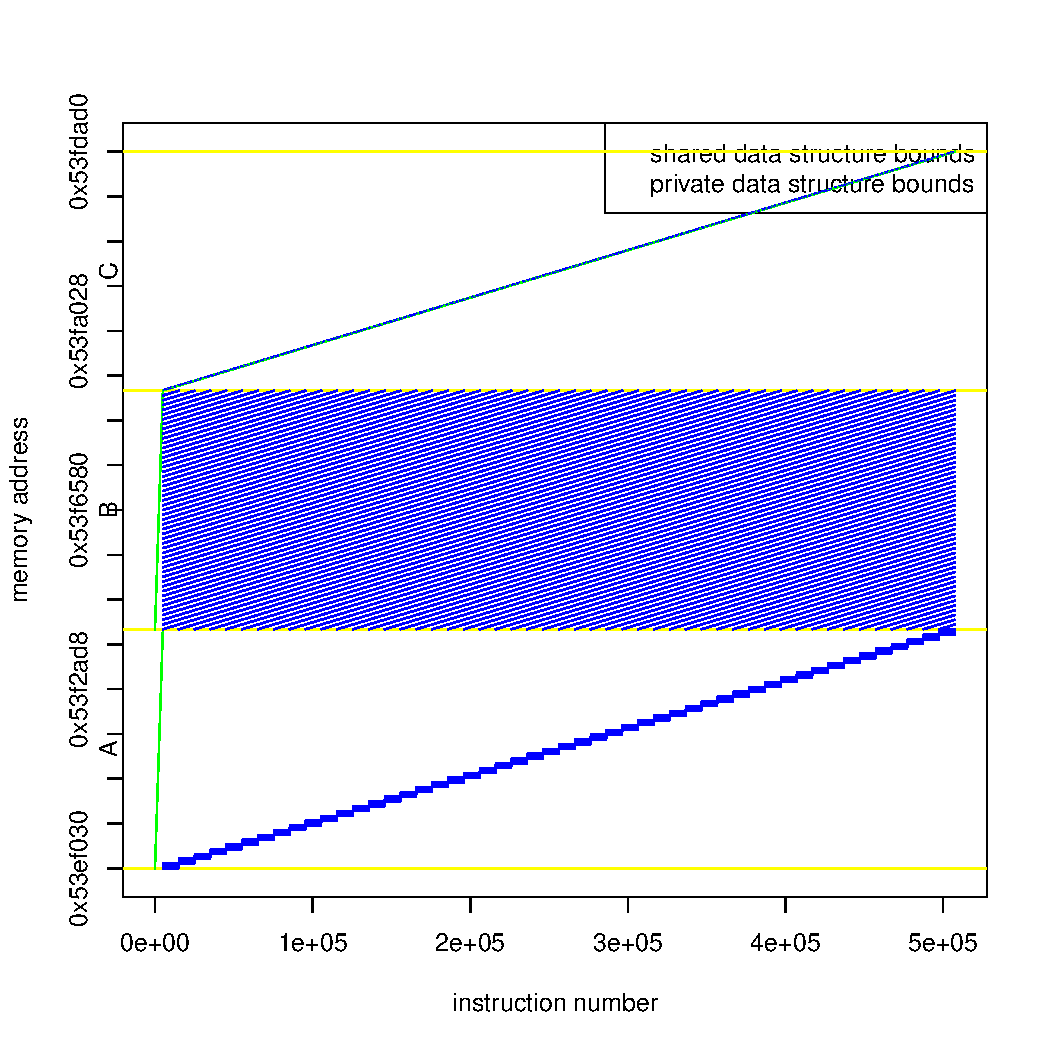
\includegraphics[width=.65\linewidth]{img/mat_naif_50_42_0_none_naif.pdf}
    \end{figure}
\end{frame}

\newsection{Conclusions and future work}

\begin{frame}{Conclusions}
    \begin{itemize}
        \item New kind of analysis
        \item Memory access patterns
        \item Temporal evolution
        \item Thread sharing informations
    \end{itemize}
\end{frame}

\newcounter{finalframe}
\setcounter{finalframe}{\value{framenumber}}
%Last numbered frame go here
\begin{frame}{Perspectives}
    \begin{itemize}
        \item Instrumentation is slow
            \begin{itemize}
                \item More efficient instrumentation tools (Pin, DynInst
                    \dots)
                \item Avoid it using a kernel module as in \cite{Cruz12Using}
            \end{itemize}
        \item Our analysis produce a lot of data
            \begin{itemize}
                \item Can we use smarter merge methods ?
                \item How can we improve the visualisation
            \end{itemize}
    \end{itemize}
\end{frame}

%=============================================================================

%=============================================================================
%Uncomment next lines for uncounted backup slides & biblio
\newHsection{Bibliography}
\setboolean{sectiontoc}{false}
%
\bibliographystyle{apalike}
\bibliography{presentation}

%========================= Backup slides =====================================
\newHsection{Hidden slides}
%put this line before each frame
\setcounter{framenumber}{\value{finalframe}}

\begin{frame}{Monothread  matrix multiplication with transposition}
    \begin{figure}
        \centering
        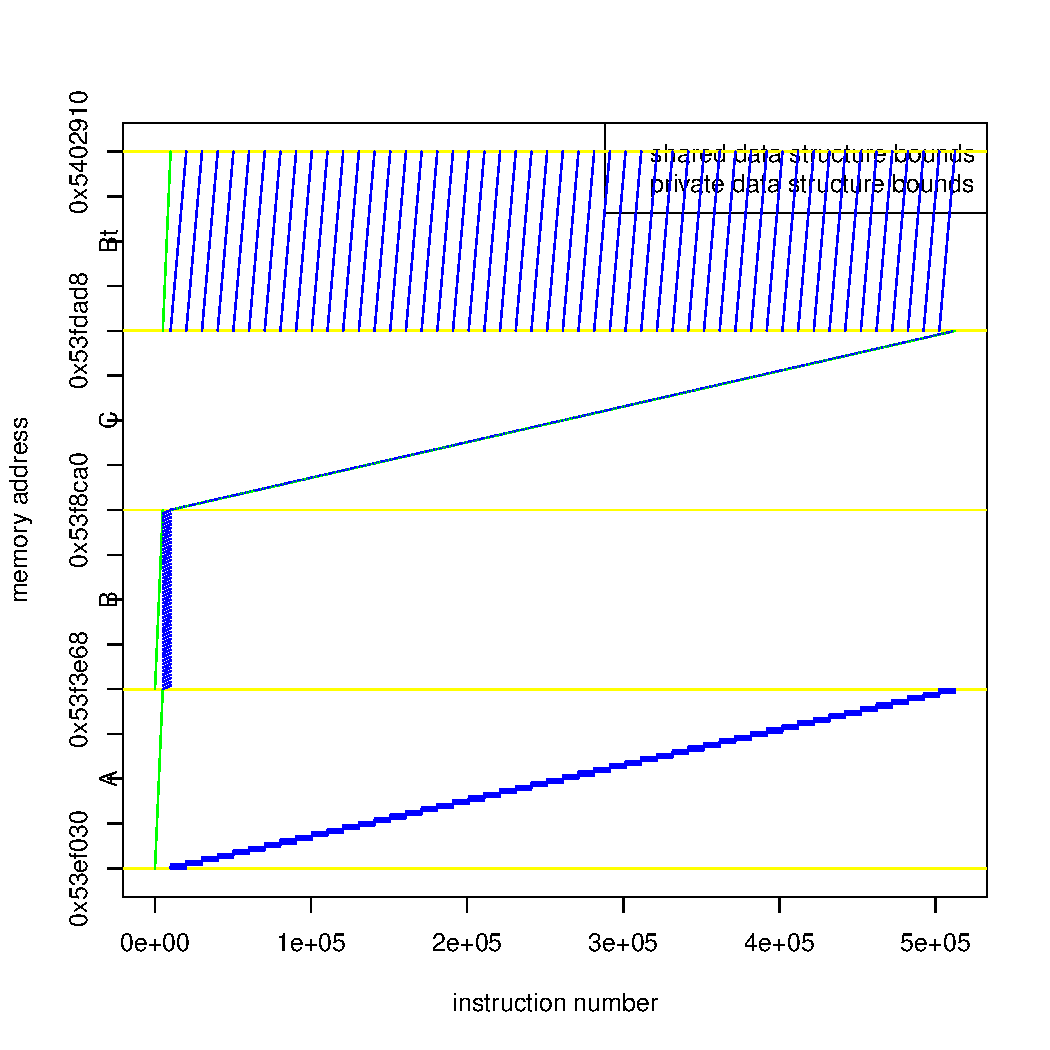
\includegraphics[width=.65\linewidth]{img/mat_naif_50_42_0_none_transpose.pdf}
    \end{figure}
\end{frame}


%=============================================================================
\end{document}


